%% Los cap'itulos inician con \chapter{T'itulo}, estos aparecen numerados y
%% se incluyen en el 'indice general.
%%
%% Recuerda que aqu'i ya puedes escribir acentos como: 'a, 'e, 'i, etc.
%% La letra n con tilde es: 'n.


\chapter{Resultados}

\section{Paquete de R \emph{geneticae}}

Una vez instalado el paquete, se debe cargar en la sesion de R mediante el comando: \textcolor{blue}{library}(geneticae). Información detallada sobre las funciones del paquete geneticae se puede obtener mediante \textcolor{blue}{help}(package = ``geneticae"). La ayuda para una función, por ejemplo \textcolor{blue}{imputation}(), en una sesión R se puede obtener usando \emph{?imputation} o \textcolor{blue}{help}(imputation). La función \textcolor{blue}{browseVignettes}(``geneticae") permite obtener la viñeta del paquete, es decir una descripción el problema que está diseñado para resolver así como ejemplos de aplicación del mismo. 

Se encuentra disponible una página web del paquete (http://....) en la que se cuenta con una breve descripción del paquete, las funciones que se incluyen en él, la viñeta, un enlace de acceso a la shiny app, entre otra información.


\subsection{Conjuntos de datos en geneticae}

El paquete geneticae contiene dos conjuntos de datos que son usados a modo de ejemplo en las funciones incluidas para analizar los datos provenientes de EMA.

\begin{itemize}[wide, nosep, labelindent = 0pt, topsep = 1ex, noitemsep,topsep=0pt]
\item \emph{yan.winterwheat dataset} (Wright, 2018): rendimiento de 18 variedades de trigo de invierno cultivadas en nueve ambientes en Ontario en 1993. A pesar de que el experimento contaba con cuatro bloques o réplicas en cada ambiente en el conjunto de datos, sólo el rendimiento medio para cada combinación de variedad y ambiente se encuentra disponible.
\begin{tcolorbox}[skin=bicolor,
    colframe=aurometalsaurus,colback=backcolour,colbacklower=white,
    width=1\linewidth,
    height=0.35\linewidth,
    boxsep=-3mm]
\begin{lstlisting}[linewidth=\columnwidth]
data(yan.winterwheat)
head(yanwinterwheat)
\end{lstlisting}

\tcblower\vskip-\baselineskip
\tcblower
\vspace{0.5cm}
\footnotesize\begin{verbatim}
##   gen  env yield
## 1 Ann BH93 4.460
## 2 Ari BH93 4.417
## 3 Aug BH93 4.669
## 4 Cas BH93 4.732
## 5 Del BH93 4.390
## 6 Dia BH93 5.178
\end{verbatim}
\end{tcolorbox}

\item \emph{plrv dataset} (CITA AGRICOLAE): rendimiento, peso de planta y parcela de 28 genotipos en 6 ubicaciones en Perú, con el fin de estudiar la resistencia a PLRV (\emph{Patato Leaf Roll Virus}) causante del enrollamiento de la hoja. Cada clon fue evaluado tres veces en cada ambiente. \\

\begin{tcolorbox}[skin=bicolor,
    colframe=aurometalsaurus,colback=backcolour,colbacklower=white,
    width=1\linewidth,
    height=0.35\linewidth,
    boxsep=-3mm]
\begin{lstlisting}
data(plrv)
head(plrv)
\end{lstlisting}

\tcblower\vskip-\baselineskip
\tcblower
\vspace{0.5cm}
\footnotesize\begin{verbatim}
##   Genotype Locality Rep WeightPlant WeightPlot    Yield
## 1   102.18     Ayac   1   0.5100000       5.10 18.88889
## 2   104.22     Ayac   1   0.3450000       2.76 12.77778
## 3   121.31     Ayac   1   0.5425000       4.34 20.09259
## 4   141.28     Ayac   1   0.9888889       8.90 36.62551
## 5   157.26     Ayac   1   0.6250000       5.00 23.14815
## 6    163.9     Ayac   1   0.5120000       2.56 18.96296
\end{verbatim}
\end{tcolorbox} 
\end{itemize}
  
\subsection{Aplicación de las funciones incluidas en el paquete}

A fin de ilustrar la metodología incluida en el paquete se utiliza el conjunto de datos \emph{yan.winterwheat}.\\

\textbf{Modelo SREG}

Para visualizar conjuntamente el efecto de G e IGA, Yan et al. (2000) propuso el biplot GGE con el cual se pueden abordar visualmente diversos aspectos relacionados con la evaluación de genotipos y ambientes. Para obtener dicho biplot en primer lugar se debe ajustar el modelo SREG mediante la función \textcolor{blue}{GGEmodel}(). 

La función \textcolor{blue}{GGEmodel}() propuesta en este paquete, es menos restrictiva que las disponibles actualmente en R en cuanto al conjunto de datos de entrada. En particular, es una modificación de la función \textcolor{blue}{GGEModel}() de GGEBiplots \textbf{(CITA)} en la que el conjunto de datos de entrada los genotipos se encuentren en las filas y los ambientes en las columnas y por lo tanto, no admite replicas. A diferencia de esto, la función \textcolor{blue}{GGEmodel}() incluida en \emph{geneticae} requiere que los datos se encuentren en formato largo, es decir las observaciones en las filas y las variables en las columnas, lo cual es más ordenado a la hora de registrar la información. Además, la base de datos puede contener otras variables que no serán utilizadas en el análisis ya que al ajustar el modelo se deben indicar en qué columnas se encuentra la información requerida por la técnica que se aplicará. Por otro lado, dado que el modelo requiere de una única observación para cada combinación de genotipo y ambiente, en caso de existir repeticiones el valor fenotípico promedio es calculado automáticamente por la función antes de ajustar el modelo. Los valores faltantes no están permitidos, en caso de haber, un mensaje de error saldrá en la consola de R.\\  

La sentencia utilizada para ajustar el modelo GGE en el conjunto de datos \emph{yan.winterwheat} se muestra a continuación. El primer argumento de la misma consiste en el nombre del \emph{dataframe} y los restantes indican los nombres que reciben las columnas que contienen la información de los genotipos, ambientes y del rasgo fenotípico de interés. Por defecto, la función considera que no hay replicas en el conjunto de datos, sin embargo, si existieran la opción \emph{rep} en la cual se indica el nombre de la columna con dicha información debe ser adicionada. Otros argumentos de dicha función son el método de centrado, de SVD y de escalado. Por defecto los datos se centran por G y GE, dando lugar al modelo SREG, otra opción en dicho argumento dará lugar a un modelo diferente. La elección del método de SVD no altera las relaciones o interacciones relativas entre los genotipos y los ambientes, aunque la apariencia del biplot será diferente, se recomienda la lectura de Yan (2002). Por último, diferentes biplots se pueden generar dependiendo del método de escalado, mayor información se encuentra disponible en Yan and Kang (2003) y Yan and Tinker (2006). En el modelo ajustado a continuación tanto el centrado, como el método SVD y de escalado son los seteados por defecto en la función.

\begin{tcolorbox}[colframe=aurometalsaurus,colback=backcolour,colbacklower=white,
   				width=1\linewidth,
    			height=0.1\linewidth,
    			boxsep=-3mm]
\begin{lstlisting}
GGE1 <- GGEmodel(yanwinterwheat, genotype = ``gen", environment = ``env", response = ``yield")
\end{lstlisting}
\end{tcolorbox}


\textbf{Biplot GGE}

La salida de la función \textcolor{blue}{GGEmodel}() es una lista que contiene las coordenadas para los genotipos y ambientes de todas las componentes, el vector de valores propios de cada componente, la variancia total, el porcentaje de variancia explicada por cada componente, entre otros. Utilizando dicha información como entrada, la función \textcolor{blue}{GGEPlot}() construye el biplot GGE. En dichos gráficos los cultivares se muestran en minúscula, para diferenciarlos de los ambientes, que están en mayúsculas. La primer componente principal se usa como la abscisa y la segunda como ordenada. Además, es posible adicionar el método de centrado, escalado y de SVD utilizado, así como también el porcentaje G + GE explicado por los dos ejes como una nota al pie del biplot con la opción \emph{footnote=T}, así como también el título del gráfico con \emph{titles = T}. 


\textbf{Comparaciones simples utilizando GGE biplot}

Dependiendo del objetivo del fitomejorador mejorador, diversos tipos de biplots GGE se pueden construir utilizando la función \textcolor{blue}{GGEPlot}(). Utilizando la opción \emph{Biplot} en el argumento \emph{type} se obtiene un biplot básico como se muestra en la figura \ref{fig:fig4121}. Se observa que explica el 78\% de la variabilidad total de G + GE. Para interpretar este gráfico se consideran los ángulos entre los vectores de los genotipos y los ambientes. Así se ve, por ejemplo, que el genotipo kat presenta un rendimiento por debajo del promedio en todos los ambientes, al tener un ángulo mayor a $90^{\circ}$ con todos los ambientes. Por otro lado, fun presenta un rendimiento por encima de la media en todos las localidades salvo en OA93 y en KE93, ya que los ángulos son agudos. La longitud de los vectores ambientales dan una medida de la capacidad del medio ambiente para discriminar entre los cultivos. 


\begin{tcolorbox}[skin=bicolor,
    colframe=aurometalsaurus,colback=backcolour,colbacklower=white,
    width=1\linewidth,
    height=0.65\linewidth,
    boxsep=-3mm]
\begin{lstlisting}
GGEPlot(GGE1, type = "Biplot", footnote = F, titles = F)
\end{lstlisting}
\tcblower\vskip-\baselineskip
\tcblower
\begin{figure}[H]
	\begin{center}
		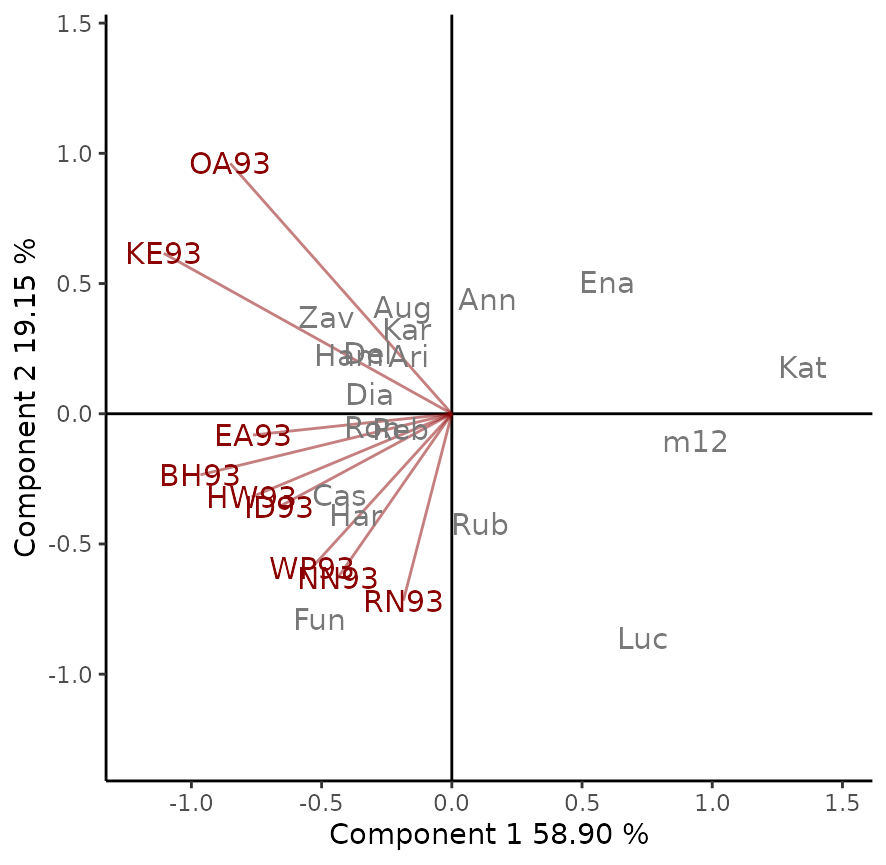
\includegraphics[width=9.5cm]{./Graficos/GGE_BIPLOT.png}
	\end{center}
	\caption{Biplot básico obtenido de la función \textcolor{blue}{GGEPlot}()}
	\label{fig:fig4121}
\end{figure}
\end{tcolorbox} 

Los mejoradores en general están interesados en identificar los cultivares más adaptados a su área, lo cual es posible a través del biplot GGE. Para esto, Yan y Hunt (2002) sugieren constituir un eje del ambiente de interés, por ejemplo OA93, trazando una recta que una el identificador del ambiente y el origen de coordenadas. Los genotipos se  clasifican en función del rendimiento en dicho ambiente de acuerdo con sus proyecciones, en la dirección indicada por el eje OA93 (Figura \ref{fig:fig4122}). Para ello, se indica la opción \emph{Selected Environment} en el argumento \emph{type} de la función y además el ambiente a evaluar en el argumento  \emph{selectedE}. Se observa en este caso que el cultivar de mayor rendimiento fue es Zav seguido por Aug, Ham, y así sucesivamente hasta llegar al genotipo Luc, que es el de menor rendimiento en ese ambiente. El eje perpendicular al del ambiente de interés, separa los genotipos con rendimiento mayor al promedio, de Zav a Cas, de aquellos con valores inferior a la media, de Ema a Luc, en OA93.
 
En forma similar, el ambiente más adecuado para un cultivar es posible determinarlo graficando una línea que una el origen de coordenadas y el marcador del genotipo de interés, por ejemplo Kat (Figura \ref{fig:fig4122}) (Yan y Hunt (2002)). Los ambientes se clasifican a lo largo del eje del genotipo en la dirección indicada por la flecha. Para obtener este gráfico la opción  \emph{Selected Genotype} debe indicarse en el argumento \emph{type}, y el genotipo de interés en  \emph{selectedG}. El eje perpendicular al del genotipo separa los ambientes en los que Kat presentó un rendimiento por debajo de su promedio, en todos los ambientes estudiados.

\begin{tcolorbox}[skin=bicolor,
    colframe=aurometalsaurus,colback=backcolour,colbacklower=white,
    width=1\linewidth,
    height=0.78\linewidth,
    boxsep=-3mm]
\begin{lstlisting}
# Ranking de cultivares en el ambiente OA93
GGEPlot(GGE1, type = "Selected Environment", selectedE = "OA93", footnote = F, titles = F)

# Ranking de ambientes para cultivar Kat
GGEPlot(GGE1, type = "Selected Genotype", selectedG = "Kat", footnote = F, titles = F)
\end{lstlisting}
\tcblower\vskip-\baselineskip
\tcblower
\begin{figure}[H]
	\begin{center}
		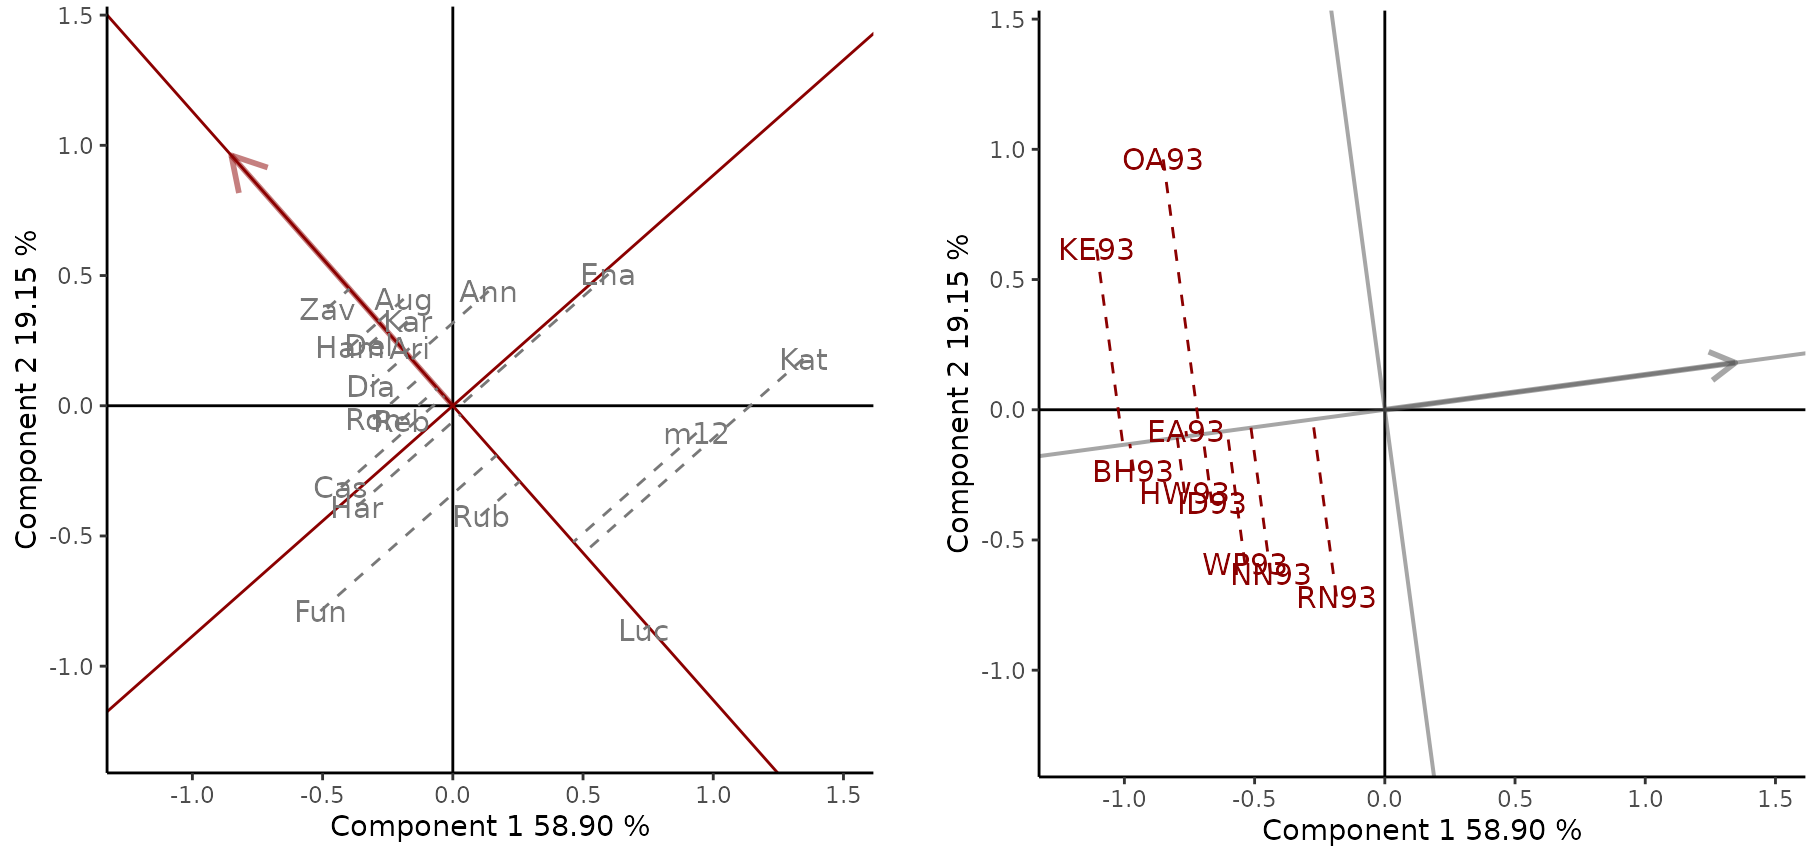
\includegraphics[width=14cm]{./Graficos/SelectedGyE.png}
	\end{center}
	\caption{A: Ranking de cultivares en el ambiente OA93. B: Ranking de ambientes para cultivar Kat}
	\label{fig:fig4122}
\end{figure}
\end{tcolorbox} 


Para comparar dos cultivares, por ejemplo Kat y Cas, una linea recta que una a los genotipos a comparar se debe trazar y luego una perpendicular a la anterior (figura \ref{fig:fig4124}). Este biplot te obtiene colocando \emph{Comparison of Genotype} en el argumento \emph{type} y los genotipos de interés en \emph{selectedG1} y \emph{selectedG2}. Se observa que todos las localidades se encuentran del mismo lado de la línea perpendicular que Cas, indicando que fue más rendidor que Kat en todos los ambientes.


\begin{tcolorbox}[skin=bicolor,
    colframe=aurometalsaurus,colback=backcolour,colbacklower=white,
    width=1\linewidth,
    height=0.65\linewidth,
    boxsep=-3mm]
\begin{lstlisting}
GGEPlot(GGE1, type = "Comparison of Genotype", selectedG1 = "Kat", selectedG2 = "Cas", footnote = F, titles = F)
\end{lstlisting}
\tcblower\vskip-\baselineskip
\tcblower
\begin{figure}[H]
	\begin{center}
		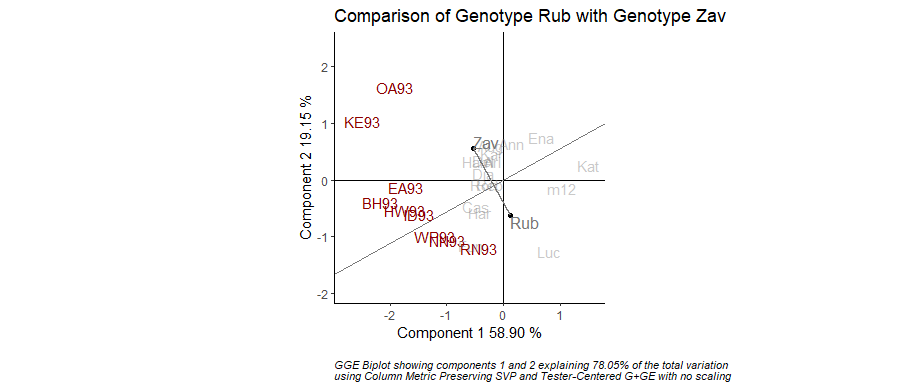
\includegraphics[width=9.5cm]{./Graficos/ComparisonofGenotype.png}
	\end{center}
	\caption{Comparación entre dos genotipos obtenido de la función \textcolor{blue}{GGEPlot}()}
	\label{fig:fig4124}
\end{figure}
\end{tcolorbox}


\textbf{Identificación de mega-ambientes con GGE biplot}

La vista poligonal del biplot GGE, obtenida al indicar \emph{Which Won Where/What} en el argumento \emph{type}, proporciona un medio eficaz de visualización del patrón ``quíen ganó dónde" de un conjunto de datos EMA (Figura \ref{fig:fig4125}).  El polígono se obtiene uniendo los cultivares (fun, zav, ena, kat y luc) que se encuentran más alejados del origen de coordenadas, de modo que todos los restantes se encuentren contenidos en el polígono. La distancia de los cultivares respecto del origen de coordenadas, en sus respectivas direcciones, es una medida de la capacidad de respuesta a los ambientes. Los ubicados en los vértices son los más alejados, por lo tanto son los cultivares que más responden, mientras que los que se encuentran en el origen de coordenadas no responden en absoluto a los ambientes estudiados.

Las perpendiculares a los lados del polígono dividen al biplot en mega-ambientes, siendo el cultivar de mayor rendimiento en todos los ambientes que se encuentran en él aquel que se encuentra en el vértice de dicho sector. Por un lado, se observa que OA93 y KE93 conforman un mega-ambiente y que Zav es el mejor cultivar. Otro está formado por el resto de los ambientes, al cual llamaremos ME1 en futuros análisis, siendo Fun el que se encuentra en el vértice. En el sector con ena, kat y luc en los vértices del polígono no se observó ningún ambiente, lo cual indica que estos cultivares fueron los menos rendidores en algunos o todos los ambientes considerados.

Se requieren dos criterios para sugerir la existencia de diferentes mega-ambientes (Gauch and Zobel, 1997). Primero, diferentes variedades superiores en los diferentes ambientes estudiados; segundo, la variación entre grupos debería ser significativamente mayor que la variación dentro del grupo.  Ambos criterios se cumplen en el presente caso (Figura \ref{fig:fig4125}). La sugerencia de dos mega-ambientes coincide con la distribución geográfica de los ambientes. La ubicación de OA (Ottawa) y KE (Kemptville) se extiende hacia el este de Ontario; BH (Bath) a pesar de pertenecer a la misma zona, tiene un clima mucho más cálido que las otras dos localidades. Las otras seis localidades consideradas se ubican al oeste o sur de la provincia.

\begin{tcolorbox}[skin=bicolor,
    colframe=aurometalsaurus,colback=backcolour,colbacklower=white,
    width=1\linewidth,
    height=0.65\linewidth,
    boxsep=-3mm]
\begin{lstlisting}
GGEPlot(GGE1, type = "Which Won Where/What", footnote = F, titles = F)
\end{lstlisting}
\tcblower\vskip-\baselineskip
\tcblower
\begin{figure}[H]
	\begin{center}
		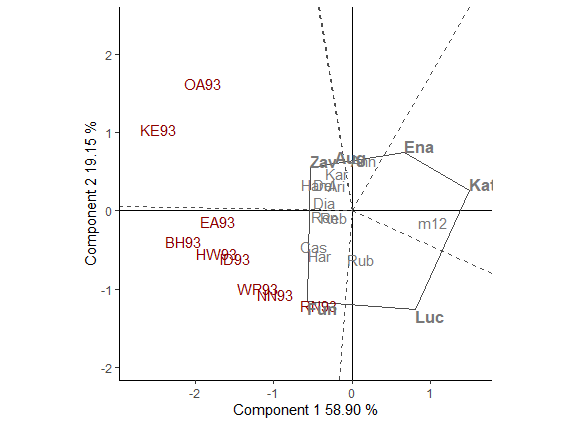
\includegraphics[width=9.5cm]{./Graficos/WhichWonWhereWhat.png}
	\end{center}
	\caption{Identificación del mejor cultivar en cada ambiente a partir de la función \textcolor{blue}{GGEPlot}()}
	\label{fig:fig4125}
\end{figure}
\end{tcolorbox}

\textbf{Evaluación de los cultivos dentro de un mega-ambientes con GGE biplot}

Una vez identificado los mega-ambientes, el siguiente paso es seleccionar cultivares dentro de cada uno de ellos. De acuerdo con la figura  \ref{fig:fig4125}, zav es el mejor cultivar para los ambientes en uno de los mega-ambiente y fun para el otro. Sin embargo, los fitomejoradores no seleccionarán un único cultivar en cada mega-ambiente, sino que es necesario evaluar todos los cultivares con el fin de conocer su desempeño (rendimiento y estabilidad).

El biplot GGE, particularmente enfocando la SVD en los genotipos, es decir utilizando el argumento \emph{SVP=row} en la función \textcolor{blue}{GGEmodel}(), proporciona un medio superior para visualizar tanto el rendimiento medio como la estabilidad de los genotipos (Figura \ref{fig:fig4126}). La visualización del rendimiento medio y la estabilidad de los genotipos a partir de un eje promedio de cada uno de los mega-ambientes formados (AEC, average environment coordinate), por ejemplo ME1, se logra indicando \emph{Mean vs. Stability} en el argumento \emph{type} (Figura \ref{fig:fig4126}). Mientras que la abscisa representa el efecto de G la ordenada el de la IGA, que es una medida de la variabilidad o inestabilidad, asociada con cada genotipo. Una mayor proyección sobre la ordenada AEC, independientemente de la dirección, significa mayor inestabilidad. Por lo tanto, rub y dia son más variables y menos estables que otros cultivares (Figura \ref{fig:fig4126}). El ambiente BH93 está ubicado en el este de Ontario caracterizado por inviernos más fríos, mientras que RN93 en el sur de Ontario caracterizado por un clima cálido y húmedo en la mayoría de los años. Esto justifica la inestabilidad de rub y dia, ya que el primero es temprano y tiene una poca resistencia al invierno por lo que se desempeñó bien en RN93 y mal en BH93, y el segundo, con un comportamiento contrario al anterior cultivar debido a que es tardío y alto. Los cultivares próximos al eje de las abscisas, cas, zav, reb, del, ari y kar, son más estables que el resto. 

Además, usando el mismo enfoque en SVD, para cada uno de los mega-ambientes identificados, es posible visualizar  el rendimiento medio y la estabilidad de los genotipos en una única medida. Un cultivar ideal es definido y a pesar de que rara vez exista, se utiliza como referencia para la evaluación de los cultivares. La distancia entre los cultivares con respecto al ideal, ubicado en el centro del conjunto de círculos concéntricos, se puede utilizar como una medida de su conveniencia. Es posible realizarlo con la función \textcolor{blue}{GGEPlot}() indicando \emph{Ranking Genotypes} en el argumento \emph{type} (Figura \ref{fig:fig4126}). Para el ME1, el cultivar fun es el más próximo al ideal, y por lo tanto, el más deseable de todos los estudiados, seguido por cas y heno, que a su vez son seguidos por ron, ham, rub, zav, del y reb, etc. (figura \ref{fig:fig4126}).


\begin{tcolorbox}[skin=bicolor,
    colframe=aurometalsaurus,colback=backcolour,colbacklower=white,
    width=1\linewidth,
    height=0.85\linewidth,
    boxsep=-3mm]
\begin{lstlisting}
# Modelo SREG enfocando SVD en los genotipos
GGE_Gpartition <- GGEmodel(ME1, genotype="gen", environment="env", response="yield", SVP="row")

# Visualizacion del rendimiento medio y la estabilidad
GGEPlot(GGE_Gpartition, type = "Mean vs. Stability", footnote = F, titles = F)

# Ranking de los genotipos respecto a uno ideal
GGEPlot(GGE_Gpartition, type = "Ranking Genotypes", footnote = F, titles = F)
\end{lstlisting}
\tcblower\vskip-\baselineskip
\tcblower
\begin{figure}[H]
	\begin{center}
		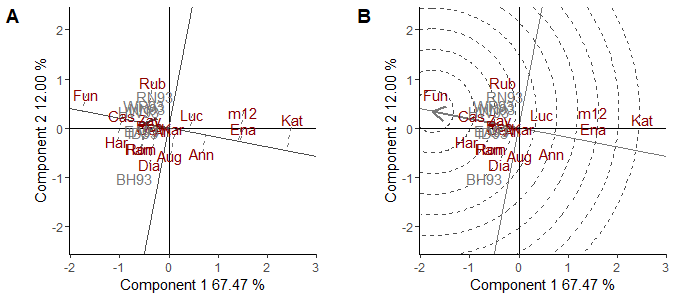
\includegraphics[width=14cm]{./Graficos/MeanvsStability2.png}
	\end{center}
	\caption{A: Evaluación de los cultivares con base en el rendimiento promedio y la estabilidad. B: Clasificación de genotipos con respecto al genotipo ideal}
	\label{fig:fig4126}
\end{figure}
\end{tcolorbox}


\textbf{Evaluación de los ambientes con GGE biplot}

A pesar de que el objetivo principal de los EMA es seleccionar cultivares también es posible evaluar los ambientes,  enfocando la SVD en los ambientes. Puede resultar de interés determinar si la región objetivo pertenece a uno o varios mega-ambientes; identificar mejores ambientes de prueba; establecer ambientes redundantes que no brindan información adicional sobre los cultivares asi como determinar ambientes que pueden usarse para la selección indirecta.

En la figura \ref{fig:fig4128} se observa que los ambientes están conectados con el origen de coordenadas a través de vectores, permitiendo comprender las interrelaciones entre los distintos ambientes del oeste y sur de Ontario que forman el mega-ambiente.  Esta visualización del biplot GGE se obtiene enfocando la SVD en los ambientes con la opción \emph{column} del argumento \emph{SVP} en \textcolor{blue}{GGEmodel}() y luego, indicando en \textcolor{blue}{GGEPlot}() \emph{Relationship Among Environments} (Figura \ref{fig:fig4128}). El coseno del ángulo entre los vectores de dos ambientes se aproxima al coeficiente de correlación entre ellos. Por ejemplo, NN93 y WP93 tienen un ángulo de aproximadamente $10^{\circ}$ entre sus vectores; por lo tanto, se encuentran estrechamente relacionados; por le contrario RN93 y OA93 presentan una correlación leve y negativa ya que el ángulo que forman sus vectores supera los $90^{\circ}$.  Por lo tanto, la Figura \ref{fig:fig4128} ayuda a identificar ambientes redundantes. Si algunos de los ambientes tienen ángulos pequeños y, por lo tanto, están altamente correlacionados, la información sobre los genotipos obtenidos de estos ambientes debe ser similar. Si esta similitud es repetible a través de los años, estos ambientes son redundantes y por lo tanto, uno solo debería ser suficiente. Obtener la misma o mejor información utilizando menos ambientes reducirá el costo y aumentará la eficiencia de producción.


La capacidad de discriminación así como la representatividad respecto del ambiente objetivo, son medidas fundamentales para un ambiente. Si no tiene capacidad de discriminación, no proporciona información sobre los cultivares y, por lo tanto, carece de utilidad. A su vez, si no es representativo no sólo que carece de utilidad sino que también puede proporcionar información sesgada sobre los cultivares evaluados. Para visualizar estas medidas, se define un ambiente promedio (AEC mencionado anteriormente) y el ambiente ideal como el centro de un conjunto de círculos concéntricos (Figura \ref{fig:fig4128}). Para obtener este biplot, se debe enfocar la SVD en los ambientes, como se indicó con anterioridad, y luego, \emph{Ranking Environments} en (\textcolor{blue}{GGEPlot}() (Figura \ref{fig:fig4128}). El ángulo entre el vector de un ambiente y el eje proporciona una medida de la representatividad. Por lo tanto, EA93 e ID93 son los más representativos, mientras que RN93 y BH93 son los menos representativos del ambiente promedio, cuando se analiza el mega-ambiente que no contiene a OA93 y a KE93 \ref{fig:fig4128}. Por otro lado, para ser discriminativo debe estar cercano al ambiente ideal. HW93 es el ambiente más cercano al ideal y, por lo tanto, es el más deseable del ME1, seguido por EA93 e ID93, que a su vez son seguidos por WP93 y NN93. RN93 y BH93 fueron los ambientes de prueba menos deseable de dicho megamabiente.




\begin{tcolorbox}[skin=bicolor,
    colframe=aurometalsaurus,colback=backcolour,colbacklower=white,
    width=1\linewidth,
    height=0.885\linewidth,
    boxsep=-3mm]
\begin{lstlisting}
# Modelo SREG enfocando SVD en los ambientes
GGE_Epartition <- GGEmodel(ME, genotype="gen", environment="env", response="yield", SVP="column")

# Relacion entre ambientes
GGEPlot(GGE_Epartition, type = "Relationship Among Environments", footnote = F, titles = F)

# Clasificacion de ambientes con respecto al ambiente ideal
GGEPlot(GGE_Epartition, type = "Ranking Environments", footnote = F, titles = F)
\end{lstlisting}
\tcblower\vskip-\baselineskip
\tcblower
\begin{figure}[H]
	\begin{center}
		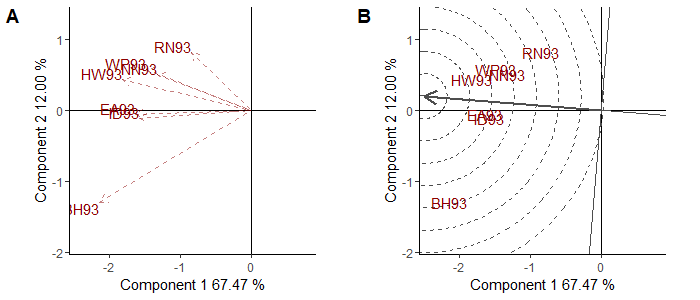
\includegraphics[width=14cm]{./Graficos/RelationshipEnvironments.png}
	\end{center}
	\caption{A:Relación entre ambientes. B:Clasificación de ambientes con respecto al ambiente ideal}
	\label{fig:fig4128}
\end{figure}
\end{tcolorbox}



\textbf{Biplot GE}

Para visualizar solamente el efecto de IGA se utiliza el biplot GE obtenido del modelo AMMI. Este gráfico es posible obtenerlo utilizando la función \textcolor{blue}{rAMMI}(), la cual no se encuentra disponible actualmente en R, y es una modificación de la publicación de Rodrigues et al. (2015). El formato del conjunto de datos de entrada es análogo al descripto en la función \textcolor{blue}{GGEmodel}(). 

El biplot clásico para el conjunto de datos \emph{yan.winterwheat} se muestra en la figura \ref{fig:fig41211} junto con la sentencia utlizada para obtener el mismo. El primer argumento es el conjunto de datos de entrada, luego se indican los nombres de las columnas en las cuales se encuentra la información necesaria para aplicar la técnica y además el biplot que se desea obtener. Se observa que la magnitud de los vectores de los ambientes BH93, KE93 y OA93 es mayor a la de los demás ambientes, es decir que son los que más contribuyen a la interacción. La cercanía de los marcadores de los genotipos m12 y Kat indica que esos genotipos tienen patrones de interacción similares, y a la vez, muy distintos a los de los genotipos Ann y Aug. Del biplot también se destacan las cercanías entre el genotipo dia y el ambiente BH93 lo que indica, debido a la gran distancia al origen, una fuerte asociación positiva entre el genotipos y el ambientes, es decir, es un ambiente muy favorable para ese genotipo.
Entre las altas asociaciones negativas se puede mencionar a la del ambiente OA93 con el genotipo Luc (marcadores opuestos en el biplot) y se interpreta que ese ambiente es considerablemente desfavorable para ese genotipo. También se observa que los genotipos Cas y Reb están próximos al origen, lo que quiere decir que se adaptan en igual medida a todos los ambientes.


\begin{tcolorbox}[skin=bicolor,
    colframe=aurometalsaurus,colback=backcolour,colbacklower=white,
    width=1\linewidth,
    height=0.7\linewidth,
    boxsep=-3mm]
\begin{lstlisting}
rAMMI(yanwinterwheat, genotype = "gen", environment = "env", response = "yield", type = "AMMI")
\end{lstlisting}
\tcblower\vskip-\baselineskip
\tcblower
\begin{figure}[H]
	\begin{center}
		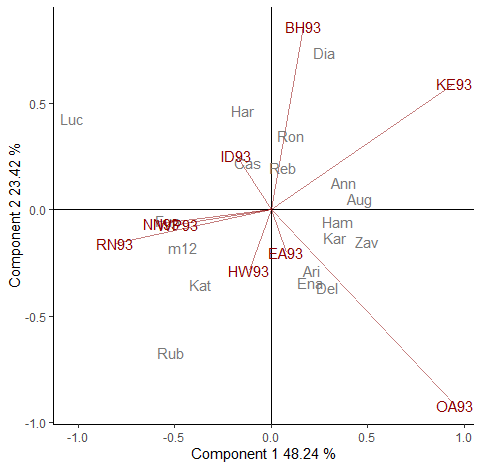
\includegraphics[width=8cm, height=7.6cm]{./Graficos/AMMI.png}
	\end{center}
	\caption{Biplot GE obtenido del modelo clasico AMMI}
	\label{fig:fig41211}
\end{figure}
\end{tcolorbox}

En caso de contar con observaciones atípicas se debe recurrir al biplot que resulta de algunos de los cinco modelos AMMI robustos propuestos por Rodrigues et al. (2015). Para ello se debe indicar en el argumento \emph{type} cuál de ellos se desea ajustar: ``rAMMI", ``hAMMI", ``gAMMI", ``lAMMI", ``ppAMMI".

Dado que el conjunto de datos \emph{yan.winterwheat} no presentan atípicas, las conclusiones obtenidas con los biplots robustos no serán muy diferentes de las realizadas con el biplot clásico (Rodrigues et al., 2015) y por lo tanto carece de sentido interpretar dichos biplots en este ejemplo. 



\textbf{Métodos de imputación}

Una limitación importante de los modelos presentados anteriormente es que requieren una que el conjunto de datos este completo, es decir que todos los genotipos sean evaluados en todos los ambientes. Por lo tanto, en el paquete se incluyen una serie de metodologías propuestas, algunas de las cuales no se encuentran disponible en R, para superar el problema de las observaciones perdidas. Entre los métodos incluidos se encuentran: ``EM-AMMI", ``EM-SVD", ``Gabriel",``WGabriel" y ``EM-PCA", los cuales se indican en la opción \emph{type} de la función \textcolor{blue}{imputation}(). El formato requerido para el conjunto de datos de entrada es análogo al indicado en las otras funciones incluidas en el paquete.

\begin{tcolorbox}[skin=bicolor,
    colframe=aurometalsaurus,colback=backcolour,colbacklower=white,
    width=1\linewidth,
    height=0.1\linewidth,
    boxsep=-3mm]
\begin{lstlisting}
imputation(yanwinterwheat, PC.nb = 2, genotype = "gen", environment = "env", response = "yield", type = "EM-AMMI")
\end{lstlisting}
\end{tcolorbox}


\section{Geneticae Shiny Web App}

Generalmente los mejoradores utilizan programas estadísticos que funcionan mediante una interfaz gráfica lo cual permite realizar el análisis de interés sin necesidad del manejo de un lenguaje de programación. \emph{Geneticae Shiny Web App}, es una aplicación web que permite a los usuarios realizar muchos de los análisis incluidos en el paquete geneticae, sin necesidad de conocer el lenguaje de programación R. 

Al iniciar \emph{Geneticae Shiny Web App}, se muestra una pantalla en la cual se carga el conjunto de datos a analizar. Se admiten archivos con extensión .csv, delimitados por coma o punto y coma.
Dado que esta aplicación se conecta con R y utiliza las funciones del paquete \emph{geneticae} se debe respetar el formato del conjunto de datos de entrada requerido por el mismo. Como se indicó anteriormente, la base de datos debe estar en formato largo, es decir que las observaciones se encuentran en las filas y las variables, genotipos, ambientes, repeticiones (en caso de que haya) y el fenotipo observado, en las columnas. Además puede incluir otras variables que no serán utilizadas en el análisis ya que al cargar el conjunto de datos se debe indicar que columna corresponde al genotipo, al ambiente, a las repeticiones y al valor fenotípico a analizar. La primera fila del conjunto de datos puede contener los nombres de las variables, y en ese caso se indicará al cargarlo en la aplicación. El número de repeticiones puede diferir con los genotipos y los ambientes.

Dos conjuntos de datos de ejemplo, \emph{plrv} y \emph{yanwinterwheat}, incluidos en el paquete geneticae, se encuentran disponibles en la aplicación para ser descargados y probar la misma (Figura \ref{fig:fig431}). La ruta para realizar esto es siguente: \emph{The data} $\rightarrow$ \emph{Example datasets}.

 \begin{figure}[H]
	\begin{center}
		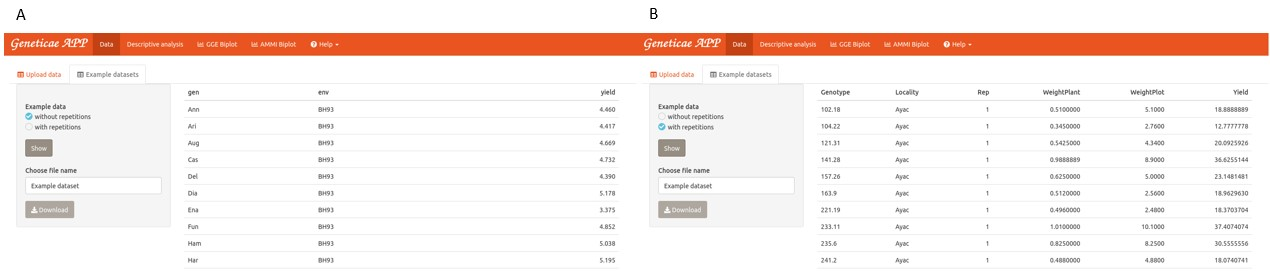
\includegraphics[width=16cm]{./Graficos/exampledata.jpg}
	\end{center}
	\caption{yanwinterwheat dataset disponible en Shiny Web App}
	\label{fig:fig431}
\end{figure}


A fin de ilustrar los diferentes análisis que se pueden realizar con esta aplicación, se utiliza el conjunto de datos \emph{yanwinterwheat} (Figura \ref{fig:fig431}). Como se dijo anteriormente, cuenta con información sobre el rendimiento medio de 18 variedades de trigo de invierno cultivadas en nueve ambientes en Ontario en 1993.


\subsection{Análisis de un caso}
En primer lugar se debe importar el conjunto de datos, indicando que el archivo .csv se encuentra delimitado por punto y coma, que la primera fila contiene los nombres de cada variable y además, el nombre de la columna que contiene la información de los genotipos, ambientes y valores fenotípicos de interés (Figura \ref{fig:fig433}). Como en este caso no se cuenta con repeticiones dicho casillero quedará sin ninguna marca. 

\begin{figure}[h]
	\begin{center}
		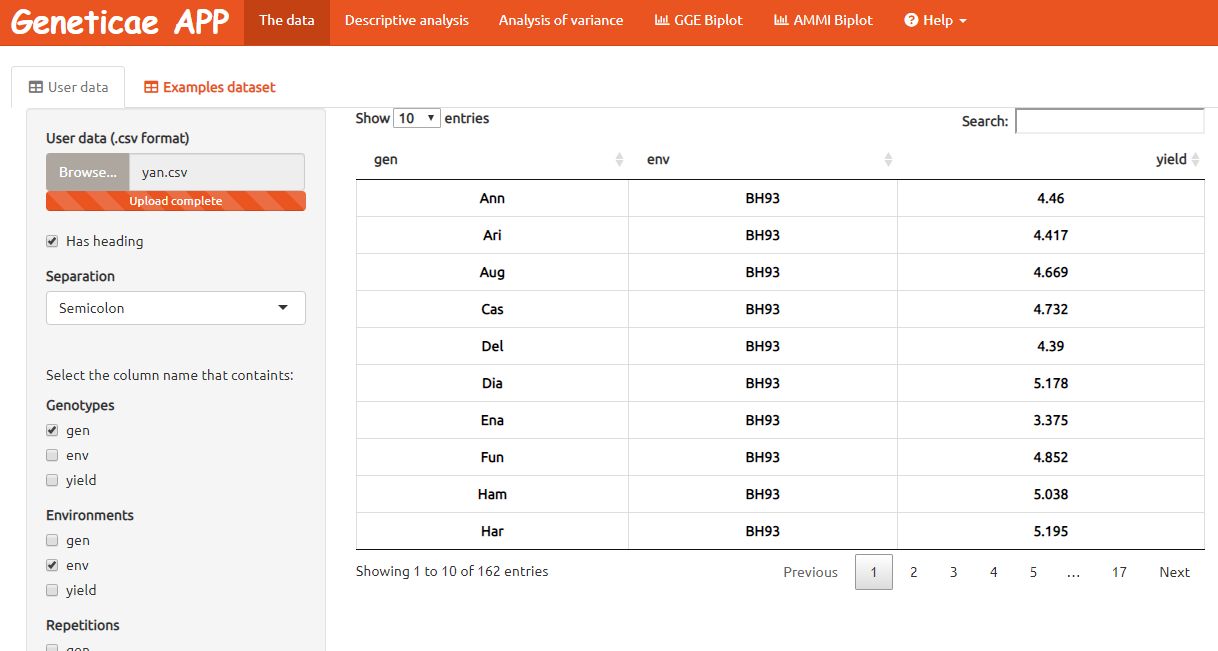
\includegraphics[width=16cm]{./Graficos/data.png}
	\end{center}
	\caption{Importar conjunto de datos}
	\label{fig:fig433}
\end{figure}


\textbf{Análisis descriptivo}

El primer paso de cualquier estudio debe ser un análisis descriptivo del conjunto de datos. La pestaña \emph{Descriptive analysis} brinda diversas herramientas para llevar a cabo dicho análisis. Una de ellas es un boxplot que compara el caracter cuantitativo de interés a través de los ambientes (Figura \ref{fig:figdesc1}) o a través de los genotipos. Este gráfico es interactivo, al posicionarse sobre cada una de las cajas se muestran las medidas resumen utilizadas para la construcción del mismo. Además los mismos se pueden descargar en formato interactivo (.HTML) al hacer click en \emph{Download} así como también en formato .png al hacer click en la cámara que aparece encima del gráfico (Figura \ref{fig:figdesc1}). Algunos aspectos estilísticos, como el color de las cajas y los nombres de los ejes, pueden ser personalizados por el usuario. 

\begin{figure}[H]
	\begin{center}
		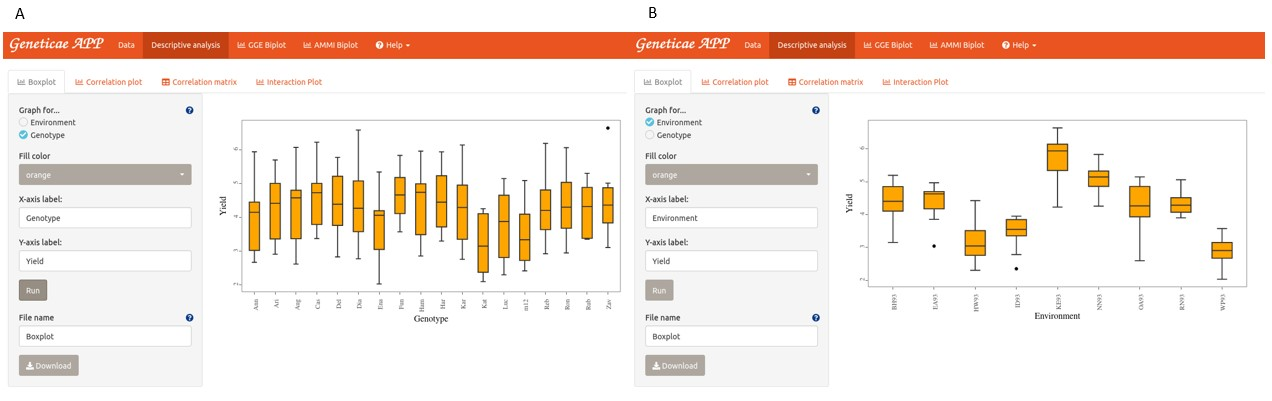
\includegraphics[width=16cm]{./Graficos/Boxplot.jpg}
	\end{center}
	\caption{Boxplot de ambientes a través de los genotipos para el conjunto de datos Plrv}
	\label{fig:figdesc1}
\end{figure}

Otro análisis de interés puede ser estudiar la correlación entre los genotipos o entre los ambientes, para ello tanto el correlograma o gráfico de correlación como la matriz de correlación se pueden realizar (Figura \ref{fig:figdesc2} y \ref{fig:figdesc3}). En ambos casos, se pueden estimar las correlaciones de Pearson o de Spearman. En el correlograma las correlaciones positivas se muestran en azul y las negativas en rojo y la intensidad del color y el tamaño del círculo son proporcionales a los coeficientes de correlación (Figura \ref{fig:figdesc2}). Dicho gráfico puede ser descargado.


\begin{figure}[H]
	\begin{center}
		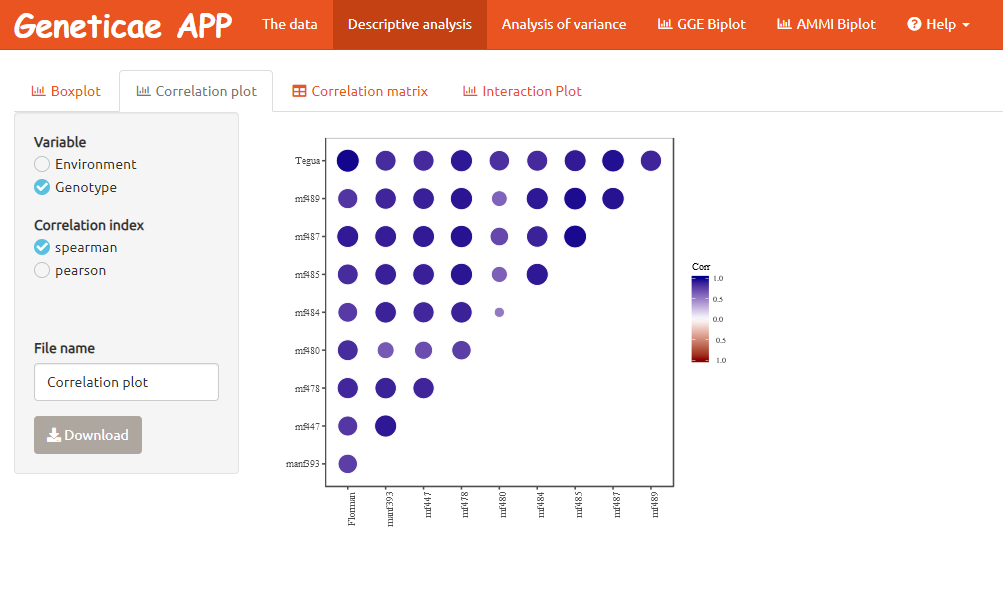
\includegraphics[width=16cm]{./Graficos/corr_gen.png}
	\end{center}
	\caption{Boxplot de genotipos a través de los ambientes para el conjunto de datos Plrv}
	\label{fig:figdesc2}
\end{figure}


\begin{figure}[H]
	\begin{center}
		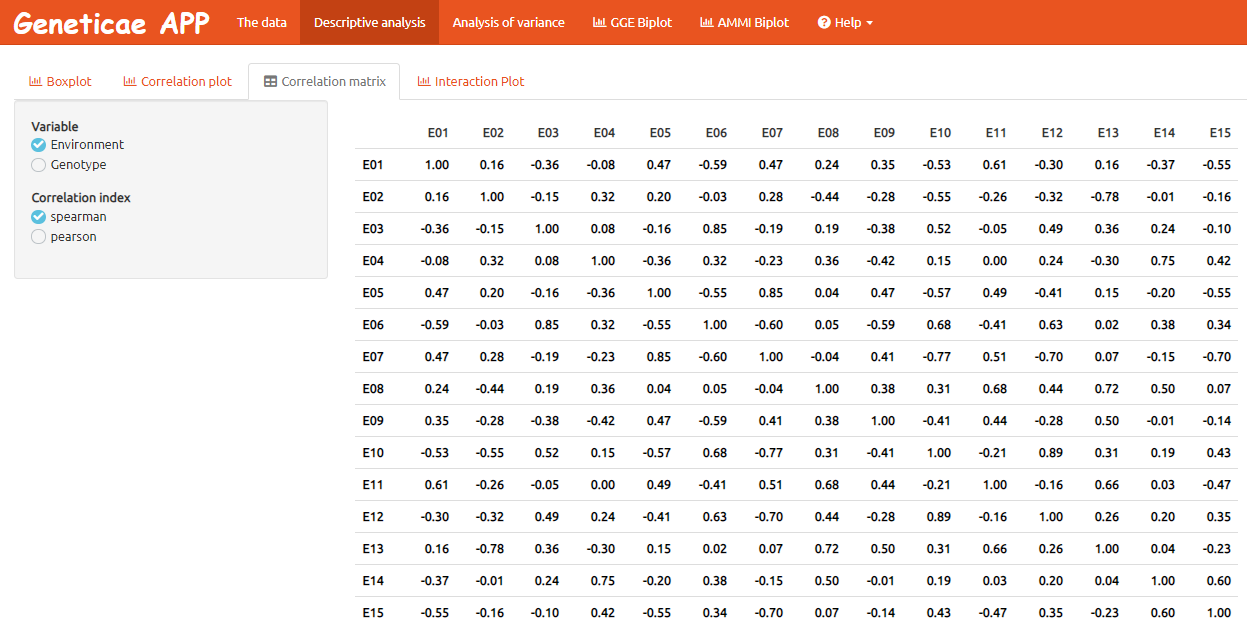
\includegraphics[width=16cm]{./Graficos/corr_matrix.png}
	\end{center}
	\caption{Boxplot de genotipos a través de los ambientes para el conjunto de datos Plrv}
	\label{fig:figdesc3}
\end{figure}



Por último, dado que inconsistencias en el rendimiento de los genotipo en diferentes ambientes complican la tarea de los fitomejoradores ya que no existe un genotipo superior en todos los ambientes estudiados y que las técnicas de principal interés de la aplicación carecen de sentido cuando dicho efecto no esta presente en el conjunto de datos, es posible realizar un gráfico de interacción. En la figura \ref{fig:figdesc4} se observa el cambio en el efecto genotípico a través de los ambientes, sin embargo es posible también mostrar el cambio en el efecto ambiental a través de los genotipos.
En forma análoga al boxplot, éste es un gráfico interactivo, y por lo tanto, es posible descargarlo en formato interactivo (.HTML) a partir del boton \emph{Download}, así como también en formato .png al hacer click en la cámara (Figura \ref{fig:figdesc4}). A su vez, los nombres de los ejes pueden ser personalizados por el usuario. 



\begin{figure}[H]
	\begin{center}
		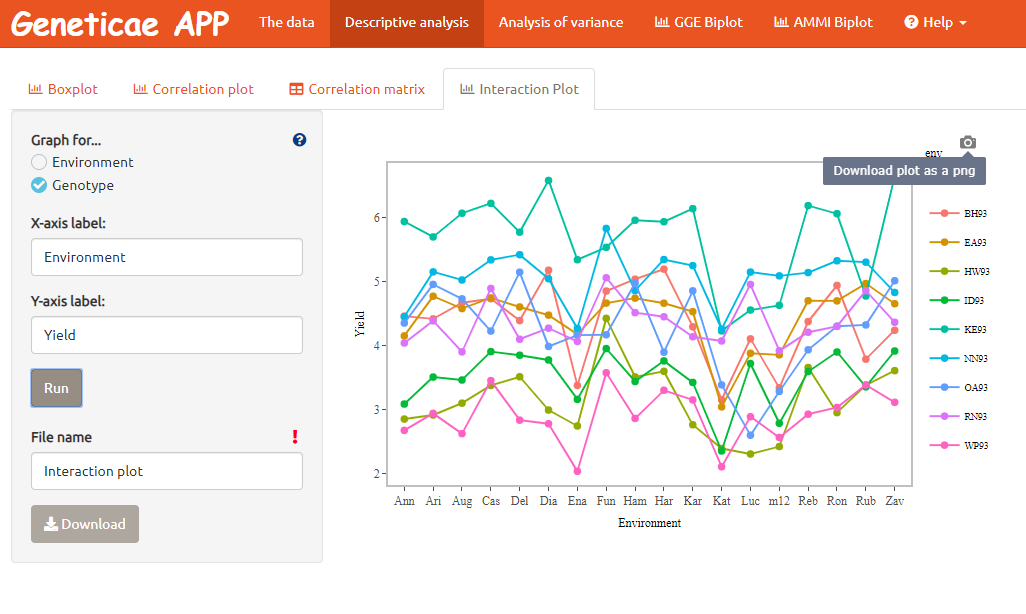
\includegraphics[width=16cm]{./Graficos/int_plot.png}
	\end{center}
	\caption{Boxplot de genotipos a través de los ambientes para el conjunto de datos Plrv}
	\label{fig:figdesc4}
\end{figure}


\textbf{Biplots}

\emph{Geneticae Shiny Web App} permite obtener tanto el biplot GGE (Figura \ref{fig:fig4312}) como el GE (Figura \ref{fig:fig4313}) . Ciertos atributos estilísticos de dichos gráficos se pueden personalizar y además pueden ser descargados.

Dada la importancia del biplot GGE, se incluyen aquellos más utilizados en el análisis de datos provenientes de EMA. Entre ellos, el biplot básico y aquellos que permiten estudiar la relación entre los ambientes (\emph{Relationship Among Environments}), la identificación del mejor cultivar en cada ambiente (\emph{Which Won Where/What}), Discrimination vs. representativeness ( \textbf{Este es el q me falta interpretar en el paquete} ), clasificación de los ambientes con respecto al ambiente ideal (\emph{Ranking Environments}), evaluación de los cultivares con base en el rendimiento promedio y la estabilidad (\emph{Mean vs. Stability}) y  clasificación de genotipos con respecto al genotipo ideal (\emph{Ranking Genotypes}). A la hora de indicar el biplot que se desea realizar se debe especificar el método de SVD, centrado y escalado correspondiente.

\begin{figure}[H]
	\begin{center}
		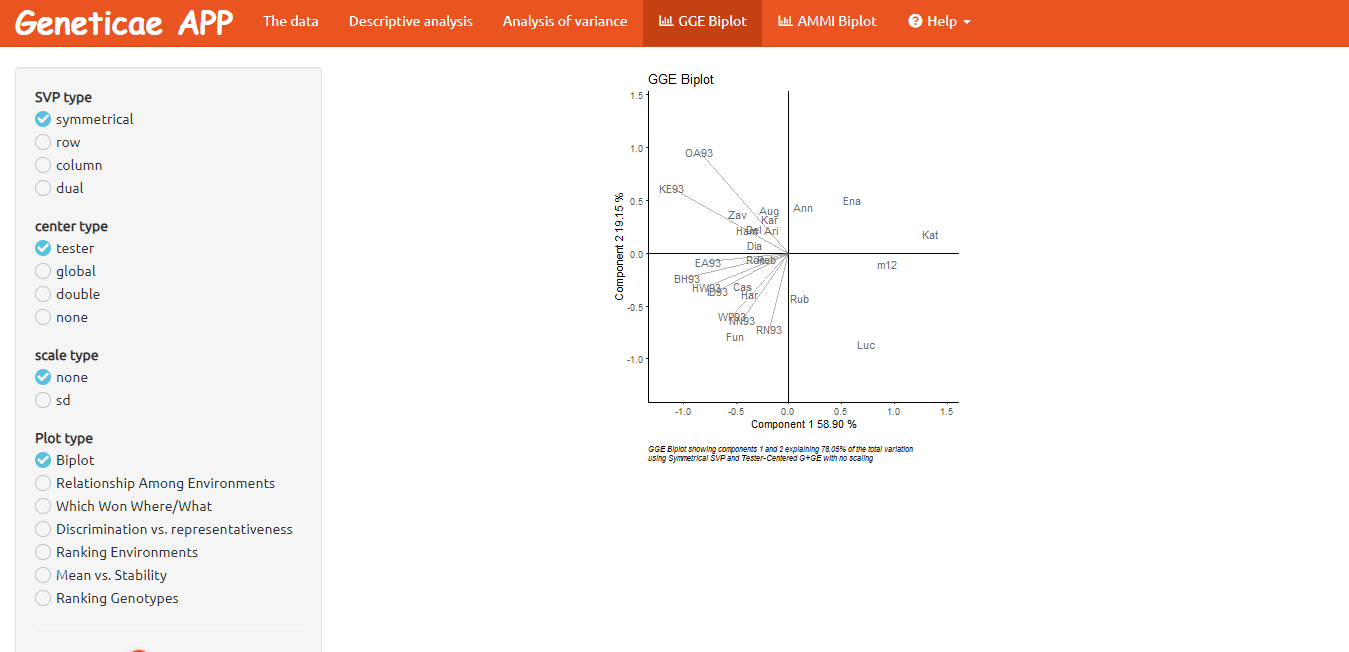
\includegraphics[width=16cm]{./Graficos/GGE.png}
	\end{center}
	\caption{Boxplot de genotipos a través de los ambientes para el conjunto de datos Plrv}
	\label{fig:fig4312}
\end{figure}


\begin{figure}[H]
	\begin{center}
		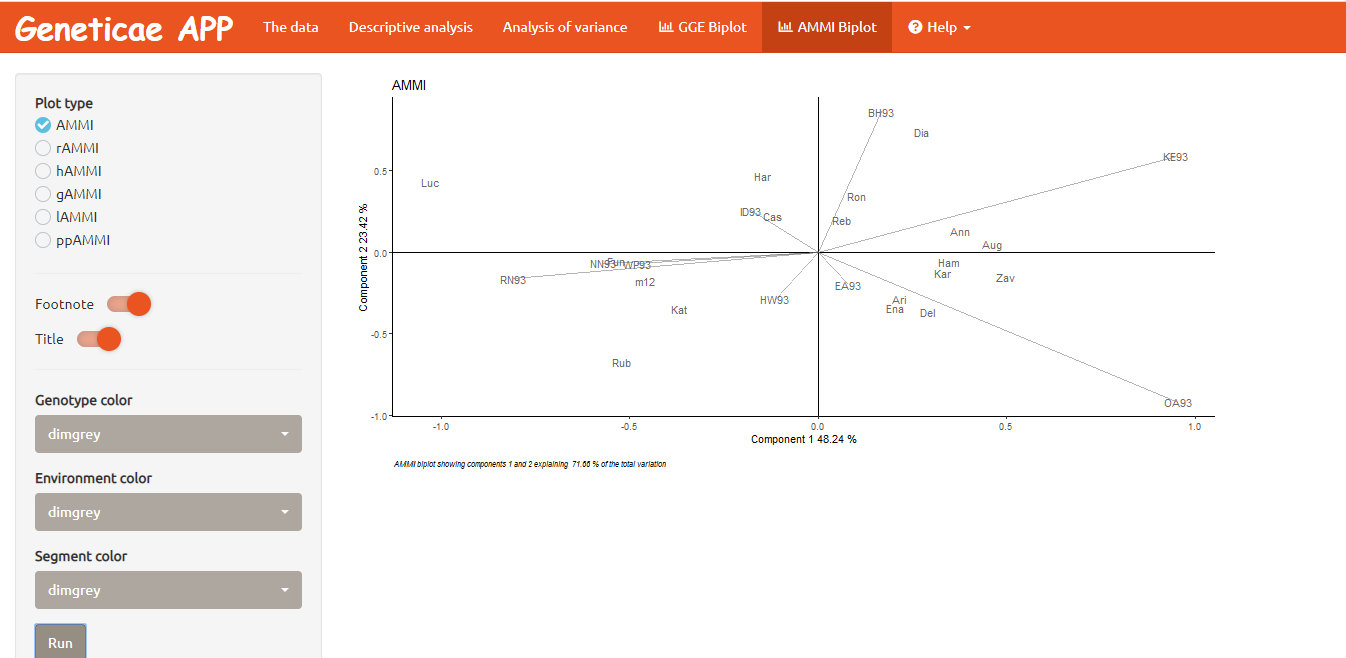
\includegraphics[width=16cm]{./Graficos/AMMI_S.png}
	\end{center}
	\caption{AMMI}
	\label{fig:fig4313}
\end{figure}



\textbf{Ayuda}

Información general, ejemplos y un video tutorial de cómo utilizar la aplicación se encuentran disponibled en la última pestaña de la misma.
